
% Default to the notebook output style

    


% Inherit from the specified cell style.




    
\documentclass[11pt]{article}

    
    
    \usepackage[T1]{fontenc}
    % Nicer default font (+ math font) than Computer Modern for most use cases
    \usepackage{mathpazo}

    % Basic figure setup, for now with no caption control since it's done
    % automatically by Pandoc (which extracts ![](path) syntax from Markdown).
    \usepackage{graphicx}
    % We will generate all images so they have a width \maxwidth. This means
    % that they will get their normal width if they fit onto the page, but
    % are scaled down if they would overflow the margins.
    \makeatletter
    \def\maxwidth{\ifdim\Gin@nat@width>\linewidth\linewidth
    \else\Gin@nat@width\fi}
    \makeatother
    \let\Oldincludegraphics\includegraphics
    % Set max figure width to be 80% of text width, for now hardcoded.
    \renewcommand{\includegraphics}[1]{\Oldincludegraphics[width=.8\maxwidth]{#1}}
    % Ensure that by default, figures have no caption (until we provide a
    % proper Figure object with a Caption API and a way to capture that
    % in the conversion process - todo).
    \usepackage{caption}
    \DeclareCaptionLabelFormat{nolabel}{}
    \captionsetup{labelformat=nolabel}

    \usepackage{adjustbox} % Used to constrain images to a maximum size 
    \usepackage{xcolor} % Allow colors to be defined
    \usepackage{enumerate} % Needed for markdown enumerations to work
    \usepackage{geometry} % Used to adjust the document margins
    \usepackage{amsmath} % Equations
    \usepackage{amssymb} % Equations
    \usepackage{textcomp} % defines textquotesingle
    % Hack from http://tex.stackexchange.com/a/47451/13684:
    \AtBeginDocument{%
        \def\PYZsq{\textquotesingle}% Upright quotes in Pygmentized code
    }
    \usepackage{upquote} % Upright quotes for verbatim code
    \usepackage{eurosym} % defines \euro
    \usepackage[mathletters]{ucs} % Extended unicode (utf-8) support
    \usepackage[utf8x]{inputenc} % Allow utf-8 characters in the tex document
    \usepackage{fancyvrb} % verbatim replacement that allows latex
    \usepackage{grffile} % extends the file name processing of package graphics 
                         % to support a larger range 
    % The hyperref package gives us a pdf with properly built
    % internal navigation ('pdf bookmarks' for the table of contents,
    % internal cross-reference links, web links for URLs, etc.)
    \usepackage{hyperref}
    \usepackage{longtable} % longtable support required by pandoc >1.10
    \usepackage{booktabs}  % table support for pandoc > 1.12.2
    \usepackage[inline]{enumitem} % IRkernel/repr support (it uses the enumerate* environment)
    \usepackage[normalem]{ulem} % ulem is needed to support strikethroughs (\sout)
                                % normalem makes italics be italics, not underlines
    

    
    
    % Colors for the hyperref package
    \definecolor{urlcolor}{rgb}{0,.145,.698}
    \definecolor{linkcolor}{rgb}{.71,0.21,0.01}
    \definecolor{citecolor}{rgb}{.12,.54,.11}

    % ANSI colors
    \definecolor{ansi-black}{HTML}{3E424D}
    \definecolor{ansi-black-intense}{HTML}{282C36}
    \definecolor{ansi-red}{HTML}{E75C58}
    \definecolor{ansi-red-intense}{HTML}{B22B31}
    \definecolor{ansi-green}{HTML}{00A250}
    \definecolor{ansi-green-intense}{HTML}{007427}
    \definecolor{ansi-yellow}{HTML}{DDB62B}
    \definecolor{ansi-yellow-intense}{HTML}{B27D12}
    \definecolor{ansi-blue}{HTML}{208FFB}
    \definecolor{ansi-blue-intense}{HTML}{0065CA}
    \definecolor{ansi-magenta}{HTML}{D160C4}
    \definecolor{ansi-magenta-intense}{HTML}{A03196}
    \definecolor{ansi-cyan}{HTML}{60C6C8}
    \definecolor{ansi-cyan-intense}{HTML}{258F8F}
    \definecolor{ansi-white}{HTML}{C5C1B4}
    \definecolor{ansi-white-intense}{HTML}{A1A6B2}

    % commands and environments needed by pandoc snippets
    % extracted from the output of `pandoc -s`
    \providecommand{\tightlist}{%
      \setlength{\itemsep}{0pt}\setlength{\parskip}{0pt}}
    \DefineVerbatimEnvironment{Highlighting}{Verbatim}{commandchars=\\\{\}}
    % Add ',fontsize=\small' for more characters per line
    \newenvironment{Shaded}{}{}
    \newcommand{\KeywordTok}[1]{\textcolor[rgb]{0.00,0.44,0.13}{\textbf{{#1}}}}
    \newcommand{\DataTypeTok}[1]{\textcolor[rgb]{0.56,0.13,0.00}{{#1}}}
    \newcommand{\DecValTok}[1]{\textcolor[rgb]{0.25,0.63,0.44}{{#1}}}
    \newcommand{\BaseNTok}[1]{\textcolor[rgb]{0.25,0.63,0.44}{{#1}}}
    \newcommand{\FloatTok}[1]{\textcolor[rgb]{0.25,0.63,0.44}{{#1}}}
    \newcommand{\CharTok}[1]{\textcolor[rgb]{0.25,0.44,0.63}{{#1}}}
    \newcommand{\StringTok}[1]{\textcolor[rgb]{0.25,0.44,0.63}{{#1}}}
    \newcommand{\CommentTok}[1]{\textcolor[rgb]{0.38,0.63,0.69}{\textit{{#1}}}}
    \newcommand{\OtherTok}[1]{\textcolor[rgb]{0.00,0.44,0.13}{{#1}}}
    \newcommand{\AlertTok}[1]{\textcolor[rgb]{1.00,0.00,0.00}{\textbf{{#1}}}}
    \newcommand{\FunctionTok}[1]{\textcolor[rgb]{0.02,0.16,0.49}{{#1}}}
    \newcommand{\RegionMarkerTok}[1]{{#1}}
    \newcommand{\ErrorTok}[1]{\textcolor[rgb]{1.00,0.00,0.00}{\textbf{{#1}}}}
    \newcommand{\NormalTok}[1]{{#1}}
    
    % Additional commands for more recent versions of Pandoc
    \newcommand{\ConstantTok}[1]{\textcolor[rgb]{0.53,0.00,0.00}{{#1}}}
    \newcommand{\SpecialCharTok}[1]{\textcolor[rgb]{0.25,0.44,0.63}{{#1}}}
    \newcommand{\VerbatimStringTok}[1]{\textcolor[rgb]{0.25,0.44,0.63}{{#1}}}
    \newcommand{\SpecialStringTok}[1]{\textcolor[rgb]{0.73,0.40,0.53}{{#1}}}
    \newcommand{\ImportTok}[1]{{#1}}
    \newcommand{\DocumentationTok}[1]{\textcolor[rgb]{0.73,0.13,0.13}{\textit{{#1}}}}
    \newcommand{\AnnotationTok}[1]{\textcolor[rgb]{0.38,0.63,0.69}{\textbf{\textit{{#1}}}}}
    \newcommand{\CommentVarTok}[1]{\textcolor[rgb]{0.38,0.63,0.69}{\textbf{\textit{{#1}}}}}
    \newcommand{\VariableTok}[1]{\textcolor[rgb]{0.10,0.09,0.49}{{#1}}}
    \newcommand{\ControlFlowTok}[1]{\textcolor[rgb]{0.00,0.44,0.13}{\textbf{{#1}}}}
    \newcommand{\OperatorTok}[1]{\textcolor[rgb]{0.40,0.40,0.40}{{#1}}}
    \newcommand{\BuiltInTok}[1]{{#1}}
    \newcommand{\ExtensionTok}[1]{{#1}}
    \newcommand{\PreprocessorTok}[1]{\textcolor[rgb]{0.74,0.48,0.00}{{#1}}}
    \newcommand{\AttributeTok}[1]{\textcolor[rgb]{0.49,0.56,0.16}{{#1}}}
    \newcommand{\InformationTok}[1]{\textcolor[rgb]{0.38,0.63,0.69}{\textbf{\textit{{#1}}}}}
    \newcommand{\WarningTok}[1]{\textcolor[rgb]{0.38,0.63,0.69}{\textbf{\textit{{#1}}}}}
    
    
    % Define a nice break command that doesn't care if a line doesn't already
    % exist.
    \def\br{\hspace*{\fill} \\* }
    % Math Jax compatability definitions
    \def\gt{>}
    \def\lt{<}
    % Document parameters
    \title{ks}
    
    
    

    % Pygments definitions
    
\makeatletter
\def\PY@reset{\let\PY@it=\relax \let\PY@bf=\relax%
    \let\PY@ul=\relax \let\PY@tc=\relax%
    \let\PY@bc=\relax \let\PY@ff=\relax}
\def\PY@tok#1{\csname PY@tok@#1\endcsname}
\def\PY@toks#1+{\ifx\relax#1\empty\else%
    \PY@tok{#1}\expandafter\PY@toks\fi}
\def\PY@do#1{\PY@bc{\PY@tc{\PY@ul{%
    \PY@it{\PY@bf{\PY@ff{#1}}}}}}}
\def\PY#1#2{\PY@reset\PY@toks#1+\relax+\PY@do{#2}}

\expandafter\def\csname PY@tok@w\endcsname{\def\PY@tc##1{\textcolor[rgb]{0.73,0.73,0.73}{##1}}}
\expandafter\def\csname PY@tok@c\endcsname{\let\PY@it=\textit\def\PY@tc##1{\textcolor[rgb]{0.25,0.50,0.50}{##1}}}
\expandafter\def\csname PY@tok@cp\endcsname{\def\PY@tc##1{\textcolor[rgb]{0.74,0.48,0.00}{##1}}}
\expandafter\def\csname PY@tok@k\endcsname{\let\PY@bf=\textbf\def\PY@tc##1{\textcolor[rgb]{0.00,0.50,0.00}{##1}}}
\expandafter\def\csname PY@tok@kp\endcsname{\def\PY@tc##1{\textcolor[rgb]{0.00,0.50,0.00}{##1}}}
\expandafter\def\csname PY@tok@kt\endcsname{\def\PY@tc##1{\textcolor[rgb]{0.69,0.00,0.25}{##1}}}
\expandafter\def\csname PY@tok@o\endcsname{\def\PY@tc##1{\textcolor[rgb]{0.40,0.40,0.40}{##1}}}
\expandafter\def\csname PY@tok@ow\endcsname{\let\PY@bf=\textbf\def\PY@tc##1{\textcolor[rgb]{0.67,0.13,1.00}{##1}}}
\expandafter\def\csname PY@tok@nb\endcsname{\def\PY@tc##1{\textcolor[rgb]{0.00,0.50,0.00}{##1}}}
\expandafter\def\csname PY@tok@nf\endcsname{\def\PY@tc##1{\textcolor[rgb]{0.00,0.00,1.00}{##1}}}
\expandafter\def\csname PY@tok@nc\endcsname{\let\PY@bf=\textbf\def\PY@tc##1{\textcolor[rgb]{0.00,0.00,1.00}{##1}}}
\expandafter\def\csname PY@tok@nn\endcsname{\let\PY@bf=\textbf\def\PY@tc##1{\textcolor[rgb]{0.00,0.00,1.00}{##1}}}
\expandafter\def\csname PY@tok@ne\endcsname{\let\PY@bf=\textbf\def\PY@tc##1{\textcolor[rgb]{0.82,0.25,0.23}{##1}}}
\expandafter\def\csname PY@tok@nv\endcsname{\def\PY@tc##1{\textcolor[rgb]{0.10,0.09,0.49}{##1}}}
\expandafter\def\csname PY@tok@no\endcsname{\def\PY@tc##1{\textcolor[rgb]{0.53,0.00,0.00}{##1}}}
\expandafter\def\csname PY@tok@nl\endcsname{\def\PY@tc##1{\textcolor[rgb]{0.63,0.63,0.00}{##1}}}
\expandafter\def\csname PY@tok@ni\endcsname{\let\PY@bf=\textbf\def\PY@tc##1{\textcolor[rgb]{0.60,0.60,0.60}{##1}}}
\expandafter\def\csname PY@tok@na\endcsname{\def\PY@tc##1{\textcolor[rgb]{0.49,0.56,0.16}{##1}}}
\expandafter\def\csname PY@tok@nt\endcsname{\let\PY@bf=\textbf\def\PY@tc##1{\textcolor[rgb]{0.00,0.50,0.00}{##1}}}
\expandafter\def\csname PY@tok@nd\endcsname{\def\PY@tc##1{\textcolor[rgb]{0.67,0.13,1.00}{##1}}}
\expandafter\def\csname PY@tok@s\endcsname{\def\PY@tc##1{\textcolor[rgb]{0.73,0.13,0.13}{##1}}}
\expandafter\def\csname PY@tok@sd\endcsname{\let\PY@it=\textit\def\PY@tc##1{\textcolor[rgb]{0.73,0.13,0.13}{##1}}}
\expandafter\def\csname PY@tok@si\endcsname{\let\PY@bf=\textbf\def\PY@tc##1{\textcolor[rgb]{0.73,0.40,0.53}{##1}}}
\expandafter\def\csname PY@tok@se\endcsname{\let\PY@bf=\textbf\def\PY@tc##1{\textcolor[rgb]{0.73,0.40,0.13}{##1}}}
\expandafter\def\csname PY@tok@sr\endcsname{\def\PY@tc##1{\textcolor[rgb]{0.73,0.40,0.53}{##1}}}
\expandafter\def\csname PY@tok@ss\endcsname{\def\PY@tc##1{\textcolor[rgb]{0.10,0.09,0.49}{##1}}}
\expandafter\def\csname PY@tok@sx\endcsname{\def\PY@tc##1{\textcolor[rgb]{0.00,0.50,0.00}{##1}}}
\expandafter\def\csname PY@tok@m\endcsname{\def\PY@tc##1{\textcolor[rgb]{0.40,0.40,0.40}{##1}}}
\expandafter\def\csname PY@tok@gh\endcsname{\let\PY@bf=\textbf\def\PY@tc##1{\textcolor[rgb]{0.00,0.00,0.50}{##1}}}
\expandafter\def\csname PY@tok@gu\endcsname{\let\PY@bf=\textbf\def\PY@tc##1{\textcolor[rgb]{0.50,0.00,0.50}{##1}}}
\expandafter\def\csname PY@tok@gd\endcsname{\def\PY@tc##1{\textcolor[rgb]{0.63,0.00,0.00}{##1}}}
\expandafter\def\csname PY@tok@gi\endcsname{\def\PY@tc##1{\textcolor[rgb]{0.00,0.63,0.00}{##1}}}
\expandafter\def\csname PY@tok@gr\endcsname{\def\PY@tc##1{\textcolor[rgb]{1.00,0.00,0.00}{##1}}}
\expandafter\def\csname PY@tok@ge\endcsname{\let\PY@it=\textit}
\expandafter\def\csname PY@tok@gs\endcsname{\let\PY@bf=\textbf}
\expandafter\def\csname PY@tok@gp\endcsname{\let\PY@bf=\textbf\def\PY@tc##1{\textcolor[rgb]{0.00,0.00,0.50}{##1}}}
\expandafter\def\csname PY@tok@go\endcsname{\def\PY@tc##1{\textcolor[rgb]{0.53,0.53,0.53}{##1}}}
\expandafter\def\csname PY@tok@gt\endcsname{\def\PY@tc##1{\textcolor[rgb]{0.00,0.27,0.87}{##1}}}
\expandafter\def\csname PY@tok@err\endcsname{\def\PY@bc##1{\setlength{\fboxsep}{0pt}\fcolorbox[rgb]{1.00,0.00,0.00}{1,1,1}{\strut ##1}}}
\expandafter\def\csname PY@tok@kc\endcsname{\let\PY@bf=\textbf\def\PY@tc##1{\textcolor[rgb]{0.00,0.50,0.00}{##1}}}
\expandafter\def\csname PY@tok@kd\endcsname{\let\PY@bf=\textbf\def\PY@tc##1{\textcolor[rgb]{0.00,0.50,0.00}{##1}}}
\expandafter\def\csname PY@tok@kn\endcsname{\let\PY@bf=\textbf\def\PY@tc##1{\textcolor[rgb]{0.00,0.50,0.00}{##1}}}
\expandafter\def\csname PY@tok@kr\endcsname{\let\PY@bf=\textbf\def\PY@tc##1{\textcolor[rgb]{0.00,0.50,0.00}{##1}}}
\expandafter\def\csname PY@tok@bp\endcsname{\def\PY@tc##1{\textcolor[rgb]{0.00,0.50,0.00}{##1}}}
\expandafter\def\csname PY@tok@fm\endcsname{\def\PY@tc##1{\textcolor[rgb]{0.00,0.00,1.00}{##1}}}
\expandafter\def\csname PY@tok@vc\endcsname{\def\PY@tc##1{\textcolor[rgb]{0.10,0.09,0.49}{##1}}}
\expandafter\def\csname PY@tok@vg\endcsname{\def\PY@tc##1{\textcolor[rgb]{0.10,0.09,0.49}{##1}}}
\expandafter\def\csname PY@tok@vi\endcsname{\def\PY@tc##1{\textcolor[rgb]{0.10,0.09,0.49}{##1}}}
\expandafter\def\csname PY@tok@vm\endcsname{\def\PY@tc##1{\textcolor[rgb]{0.10,0.09,0.49}{##1}}}
\expandafter\def\csname PY@tok@sa\endcsname{\def\PY@tc##1{\textcolor[rgb]{0.73,0.13,0.13}{##1}}}
\expandafter\def\csname PY@tok@sb\endcsname{\def\PY@tc##1{\textcolor[rgb]{0.73,0.13,0.13}{##1}}}
\expandafter\def\csname PY@tok@sc\endcsname{\def\PY@tc##1{\textcolor[rgb]{0.73,0.13,0.13}{##1}}}
\expandafter\def\csname PY@tok@dl\endcsname{\def\PY@tc##1{\textcolor[rgb]{0.73,0.13,0.13}{##1}}}
\expandafter\def\csname PY@tok@s2\endcsname{\def\PY@tc##1{\textcolor[rgb]{0.73,0.13,0.13}{##1}}}
\expandafter\def\csname PY@tok@sh\endcsname{\def\PY@tc##1{\textcolor[rgb]{0.73,0.13,0.13}{##1}}}
\expandafter\def\csname PY@tok@s1\endcsname{\def\PY@tc##1{\textcolor[rgb]{0.73,0.13,0.13}{##1}}}
\expandafter\def\csname PY@tok@mb\endcsname{\def\PY@tc##1{\textcolor[rgb]{0.40,0.40,0.40}{##1}}}
\expandafter\def\csname PY@tok@mf\endcsname{\def\PY@tc##1{\textcolor[rgb]{0.40,0.40,0.40}{##1}}}
\expandafter\def\csname PY@tok@mh\endcsname{\def\PY@tc##1{\textcolor[rgb]{0.40,0.40,0.40}{##1}}}
\expandafter\def\csname PY@tok@mi\endcsname{\def\PY@tc##1{\textcolor[rgb]{0.40,0.40,0.40}{##1}}}
\expandafter\def\csname PY@tok@il\endcsname{\def\PY@tc##1{\textcolor[rgb]{0.40,0.40,0.40}{##1}}}
\expandafter\def\csname PY@tok@mo\endcsname{\def\PY@tc##1{\textcolor[rgb]{0.40,0.40,0.40}{##1}}}
\expandafter\def\csname PY@tok@ch\endcsname{\let\PY@it=\textit\def\PY@tc##1{\textcolor[rgb]{0.25,0.50,0.50}{##1}}}
\expandafter\def\csname PY@tok@cm\endcsname{\let\PY@it=\textit\def\PY@tc##1{\textcolor[rgb]{0.25,0.50,0.50}{##1}}}
\expandafter\def\csname PY@tok@cpf\endcsname{\let\PY@it=\textit\def\PY@tc##1{\textcolor[rgb]{0.25,0.50,0.50}{##1}}}
\expandafter\def\csname PY@tok@c1\endcsname{\let\PY@it=\textit\def\PY@tc##1{\textcolor[rgb]{0.25,0.50,0.50}{##1}}}
\expandafter\def\csname PY@tok@cs\endcsname{\let\PY@it=\textit\def\PY@tc##1{\textcolor[rgb]{0.25,0.50,0.50}{##1}}}

\def\PYZbs{\char`\\}
\def\PYZus{\char`\_}
\def\PYZob{\char`\{}
\def\PYZcb{\char`\}}
\def\PYZca{\char`\^}
\def\PYZam{\char`\&}
\def\PYZlt{\char`\<}
\def\PYZgt{\char`\>}
\def\PYZsh{\char`\#}
\def\PYZpc{\char`\%}
\def\PYZdl{\char`\$}
\def\PYZhy{\char`\-}
\def\PYZsq{\char`\'}
\def\PYZdq{\char`\"}
\def\PYZti{\char`\~}
% for compatibility with earlier versions
\def\PYZat{@}
\def\PYZlb{[}
\def\PYZrb{]}
\makeatother


    % Exact colors from NB
    \definecolor{incolor}{rgb}{0.0, 0.0, 0.5}
    \definecolor{outcolor}{rgb}{0.545, 0.0, 0.0}



    
    % Prevent overflowing lines due to hard-to-break entities
    \sloppy 
    % Setup hyperref package
    \hypersetup{
      breaklinks=true,  % so long urls are correctly broken across lines
      colorlinks=true,
      urlcolor=urlcolor,
      linkcolor=linkcolor,
      citecolor=citecolor,
      }
    % Slightly bigger margins than the latex defaults
    
    \geometry{verbose,tmargin=1in,bmargin=1in,lmargin=1in,rmargin=1in}
    
    

    \begin{document}
    
    
    \maketitle
    
    

    
    \section{The Karplus-Strong
Algorithm}\label{the-karplus-strong-algorithm}

The Karplus-Strong algorithm is a simple digital feedback loop with an
internal buffer of \(M\) samples. The buffer is filled with a set of
initial values and the loop, when running, produces an arbitraryly long
output signal. Although elementary, the K-S loop can be used to
synthesize interesting musical sounds as we will see in this notebook.

Let's start with a basic implementation of the K-S loop:

    \begin{Verbatim}[commandchars=\\\{\}]
{\color{incolor}In [{\color{incolor}1}]:} \PY{k}{def} \PY{n+nf}{KS\PYZus{}1}\PY{p}{(}\PY{n}{x}\PY{p}{,} \PY{n}{N}\PY{p}{)}\PY{p}{:}
            \PY{c+c1}{\PYZsh{} given the initial buffer x, produce a N\PYZhy{}sample output}
            \PY{c+c1}{\PYZsh{}  by concatenating identical copies of the buffer}
            \PY{n}{y} \PY{o}{=} \PY{n}{x}
            \PY{k}{while} \PY{n+nb}{len}\PY{p}{(}\PY{n}{y}\PY{p}{)} \PY{o}{\PYZlt{}} \PY{n}{N}\PY{p}{:}
                \PY{c+c1}{\PYZsh{} keep appending until we reach or exceed the required length}
                \PY{n}{y} \PY{o}{=} \PY{n}{np}\PY{o}{.}\PY{n}{append}\PY{p}{(}\PY{n}{y}\PY{p}{,} \PY{n}{x}\PY{p}{)}
            \PY{c+c1}{\PYZsh{} trim the excess}
            \PY{n}{y} \PY{o}{=} \PY{n}{y}\PY{p}{[}\PY{l+m+mi}{0}\PY{p}{:}\PY{n}{N}\PY{o}{+}\PY{l+m+mi}{1}\PY{p}{]}
            \PY{k}{return} \PY{n}{y}
\end{Verbatim}


    OK, let's try it out right away! Yet, however impatient we may be, we
still need to do a few things. First we need to include the necessary
Python libraries:

    \begin{Verbatim}[commandchars=\\\{\}]
{\color{incolor}In [{\color{incolor}2}]:} \PY{o}{\PYZpc{}}\PY{k}{matplotlib} inline
        \PY{k+kn}{import} \PY{n+nn}{matplotlib}
        \PY{k+kn}{import} \PY{n+nn}{matplotlib}\PY{n+nn}{.}\PY{n+nn}{pyplot} \PY{k}{as} \PY{n+nn}{plt}
        \PY{k+kn}{import} \PY{n+nn}{numpy} \PY{k}{as} \PY{n+nn}{np}
        \PY{k+kn}{import} \PY{n+nn}{IPython}
\end{Verbatim}


    \begin{Verbatim}[commandchars=\\\{\}]
{\color{incolor}In [{\color{incolor}3}]:} \PY{n}{plt}\PY{o}{.}\PY{n}{rcParams}\PY{p}{[}\PY{l+s+s2}{\PYZdq{}}\PY{l+s+s2}{figure.figsize}\PY{l+s+s2}{\PYZdq{}}\PY{p}{]} \PY{o}{=} \PY{p}{(}\PY{l+m+mi}{14}\PY{p}{,}\PY{l+m+mi}{4}\PY{p}{)}
\end{Verbatim}


    Then, since we're playing audio, we need to set the internal "clock" of
the system, aka the sampling rate:

    \begin{Verbatim}[commandchars=\\\{\}]
{\color{incolor}In [{\color{incolor}4}]:} \PY{n}{Fs} \PY{o}{=} \PY{l+m+mi}{16000} \PY{c+c1}{\PYZsh{} 16 KHz sampling rate}
\end{Verbatim}


    With this sampling rate, since the period of the generated signal is
equal to the length of the inital buffer, we will be able to compute the
fundamental frequency of the resulting sound. For instance, if we init
the K-S algorithm with a vector of 50 values, the buffer will fit
\(16000 / 50 = 320\) times in a second's worth of samples or, in other
words, the resulting frequency will be 320Hz, which corresponds roughly
to a E4 on a piano.

We still haven't talked about what to use as the initial values for the
buffer. Well, the cool thing about K-S is that we can use pretty much
anything we want; as a matter of fact, using random values will give you
a totally fine sound. As a proof, consider this initial data set:

    \begin{Verbatim}[commandchars=\\\{\}]
{\color{incolor}In [{\color{incolor}5}]:} \PY{n}{b} \PY{o}{=} \PY{n}{np}\PY{o}{.}\PY{n}{random}\PY{o}{.}\PY{n}{randn}\PY{p}{(}\PY{l+m+mi}{50}\PY{p}{)}
        \PY{n}{plt}\PY{o}{.}\PY{n}{stem}\PY{p}{(}\PY{n}{b}\PY{p}{)}\PY{p}{;}
\end{Verbatim}


    \begin{center}
    \adjustimage{max size={0.9\linewidth}{0.9\paperheight}}{output_8_0.png}
    \end{center}
    { \hspace*{\fill} \\}
    
    Let's now generate a 2-second audio clip:

    \begin{Verbatim}[commandchars=\\\{\}]
{\color{incolor}In [{\color{incolor}6}]:} \PY{n}{y} \PY{o}{=} \PY{n}{KS\PYZus{}1}\PY{p}{(}\PY{n}{b}\PY{p}{,} \PY{n}{Fs} \PY{o}{*} \PY{l+m+mi}{2}\PY{p}{)}
        
        \PY{c+c1}{\PYZsh{} we can look at a few periods:}
        \PY{n}{plt}\PY{o}{.}\PY{n}{stem}\PY{p}{(}\PY{n}{y}\PY{p}{[}\PY{l+m+mi}{0}\PY{p}{:}\PY{l+m+mi}{500}\PY{p}{]}\PY{p}{)}\PY{p}{;}
\end{Verbatim}


    \begin{center}
    \adjustimage{max size={0.9\linewidth}{0.9\paperheight}}{output_10_0.png}
    \end{center}
    { \hspace*{\fill} \\}
    
    \begin{Verbatim}[commandchars=\\\{\}]
{\color{incolor}In [{\color{incolor}7}]:} \PY{n}{IPython}\PY{o}{.}\PY{n}{display}\PY{o}{.}\PY{n}{Audio}\PY{p}{(}\PY{n}{y}\PY{p}{,} \PY{n}{rate}\PY{o}{=}\PY{n}{Fs}\PY{p}{)}
\end{Verbatim}


\begin{Verbatim}[commandchars=\\\{\}]
{\color{outcolor}Out[{\color{outcolor}7}]:} <IPython.lib.display.Audio object>
\end{Verbatim}
            
    \begin{Verbatim}[commandchars=\\\{\}]
{\color{incolor}In [{\color{incolor}8}]:} \PY{c+c1}{\PYZsh{} let\PYZsq{}s play an octave lower: just double the initial buffer\PYZsq{}s length}
        \PY{n}{IPython}\PY{o}{.}\PY{n}{display}\PY{o}{.}\PY{n}{Audio}\PY{p}{(}\PY{n}{KS\PYZus{}1}\PY{p}{(}\PY{n}{np}\PY{o}{.}\PY{n}{random}\PY{o}{.}\PY{n}{rand}\PY{p}{(}\PY{l+m+mi}{100}\PY{p}{)}\PY{p}{,} \PY{n}{Fs} \PY{o}{*} \PY{l+m+mi}{2}\PY{p}{)}\PY{p}{,} \PY{n}{rate}\PY{o}{=}\PY{n}{Fs}\PY{p}{)}
\end{Verbatim}


\begin{Verbatim}[commandchars=\\\{\}]
{\color{outcolor}Out[{\color{outcolor}8}]:} <IPython.lib.display.Audio object>
\end{Verbatim}
            
    OK, so the K-S algorithm works! From the signal processing point of
view, we can describe the system with the following block diagram
(neglect the factor \(\alpha\) for a moment)

\begin{figure}
\centering
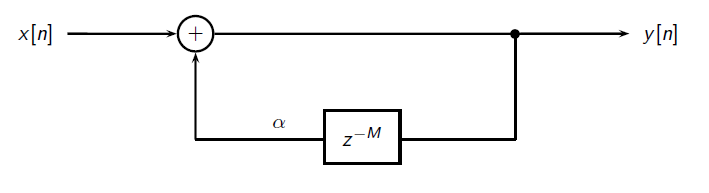
\includegraphics{ks.png}
\caption{title}
\end{figure}

The output can be expressed as \[
    y[n] = x[n] + y[n - M]
\] assuming that the input is the finite-support signal \[
x[n] = \begin{cases}
    0 & \mbox{for $n < 0$} \\
    b_n & \mbox{for $0 \le n < M$} \\
    0 & \mbox{for $n \ge M$}
  \end{cases}
\]

Let's implement the K-S algorithm as a signal processing loop

    \begin{Verbatim}[commandchars=\\\{\}]
{\color{incolor}In [{\color{incolor}9}]:} \PY{k}{def} \PY{n+nf}{KS\PYZus{}2}\PY{p}{(}\PY{n}{x}\PY{p}{,} \PY{n}{N}\PY{p}{)}\PY{p}{:}
            \PY{c+c1}{\PYZsh{} length of the input}
            \PY{n}{M} \PY{o}{=} \PY{n+nb}{len}\PY{p}{(}\PY{n}{x}\PY{p}{)}
            \PY{c+c1}{\PYZsh{} prepare the output}
            \PY{n}{y} \PY{o}{=} \PY{n}{np}\PY{o}{.}\PY{n}{zeros}\PY{p}{(}\PY{n}{N}\PY{p}{)}
            \PY{c+c1}{\PYZsh{} this is NOT an efficient implementation, but it shows the general principle}
            \PY{c+c1}{\PYZsh{} we assume zero initial conditions (y[n]=0 for n \PYZlt{} 0)}
            \PY{k}{for} \PY{n}{n} \PY{o+ow}{in} \PY{n+nb}{range}\PY{p}{(}\PY{l+m+mi}{0}\PY{p}{,} \PY{n}{N}\PY{p}{)}\PY{p}{:}
                \PY{n}{y}\PY{p}{[}\PY{n}{n}\PY{p}{]} \PY{o}{=} \PY{p}{(}\PY{n}{x}\PY{p}{[}\PY{n}{n}\PY{p}{]} \PY{k}{if} \PY{n}{n} \PY{o}{\PYZlt{}} \PY{n}{M} \PY{k}{else} \PY{l+m+mi}{0}\PY{p}{)} \PY{o}{+} \PY{p}{(}\PY{n}{y}\PY{p}{[}\PY{n}{n}\PY{o}{\PYZhy{}}\PY{n}{M}\PY{p}{]} \PY{k}{if} \PY{n}{n}\PY{o}{\PYZhy{}}\PY{n}{M} \PY{o}{\PYZgt{}}\PY{o}{=} \PY{l+m+mi}{0} \PY{k}{else} \PY{l+m+mi}{0}\PY{p}{)}
            \PY{k}{return} \PY{n}{y}
\end{Verbatim}


    \begin{Verbatim}[commandchars=\\\{\}]
{\color{incolor}In [{\color{incolor}10}]:} \PY{c+c1}{\PYZsh{} it should still work}
         \PY{n}{IPython}\PY{o}{.}\PY{n}{display}\PY{o}{.}\PY{n}{Audio}\PY{p}{(}\PY{n}{KS\PYZus{}2}\PY{p}{(}\PY{n}{np}\PY{o}{.}\PY{n}{random}\PY{o}{.}\PY{n}{rand}\PY{p}{(}\PY{l+m+mi}{50}\PY{p}{)}\PY{p}{,} \PY{n}{Fs} \PY{o}{*} \PY{l+m+mi}{2}\PY{p}{)}\PY{p}{,} \PY{n}{rate}\PY{o}{=}\PY{n}{Fs}\PY{p}{)}
\end{Verbatim}


\begin{Verbatim}[commandchars=\\\{\}]
{\color{outcolor}Out[{\color{outcolor}10}]:} <IPython.lib.display.Audio object>
\end{Verbatim}
            
    By looking at block diagram we can see a simple modification that adds a
lot of realism to the sound: by setting \(\alpha\) to a value close to
but less that one, we can introuce a decay in the note that produces
guitar-like sounds: \[
    y[n] = x[n] + \alpha y[n - M]
\]

    \begin{Verbatim}[commandchars=\\\{\}]
{\color{incolor}In [{\color{incolor}11}]:} \PY{k}{def} \PY{n+nf}{KS\PYZus{}3}\PY{p}{(}\PY{n}{x}\PY{p}{,} \PY{n}{N}\PY{p}{,} \PY{n}{alpha} \PY{o}{=} \PY{l+m+mf}{0.99}\PY{p}{)}\PY{p}{:}
             \PY{n}{M} \PY{o}{=} \PY{n+nb}{len}\PY{p}{(}\PY{n}{x}\PY{p}{)}
             \PY{n}{y} \PY{o}{=} \PY{n}{np}\PY{o}{.}\PY{n}{zeros}\PY{p}{(}\PY{n}{N}\PY{p}{)}
             \PY{c+c1}{\PYZsh{} }
             \PY{k}{for} \PY{n}{n} \PY{o+ow}{in} \PY{n+nb}{range}\PY{p}{(}\PY{l+m+mi}{0}\PY{p}{,} \PY{n}{N}\PY{p}{)}\PY{p}{:}
                 \PY{n}{y}\PY{p}{[}\PY{n}{n}\PY{p}{]} \PY{o}{=} \PY{p}{(}\PY{n}{x}\PY{p}{[}\PY{n}{n}\PY{p}{]} \PY{k}{if} \PY{n}{n} \PY{o}{\PYZlt{}} \PY{n}{M} \PY{k}{else} \PY{l+m+mi}{0}\PY{p}{)} \PY{o}{+} \PY{n}{alpha} \PY{o}{*} \PY{p}{(}\PY{n}{y}\PY{p}{[}\PY{n}{n}\PY{o}{\PYZhy{}}\PY{n}{M}\PY{p}{]} \PY{k}{if} \PY{n}{n}\PY{o}{\PYZhy{}}\PY{n}{M} \PY{o}{\PYZgt{}}\PY{o}{=} \PY{l+m+mi}{0} \PY{k}{else} \PY{l+m+mi}{0}\PY{p}{)}
             \PY{k}{return} \PY{n}{y}
\end{Verbatim}


    If we now plot the resulting K-S output, we can see the decaying
envelope:

    \begin{Verbatim}[commandchars=\\\{\}]
{\color{incolor}In [{\color{incolor}12}]:} \PY{n}{y} \PY{o}{=} \PY{n}{KS\PYZus{}3}\PY{p}{(}\PY{n}{b}\PY{p}{,} \PY{n}{Fs} \PY{o}{*} \PY{l+m+mi}{2}\PY{p}{)}
         \PY{n}{plt}\PY{o}{.}\PY{n}{stem}\PY{p}{(}\PY{n}{y}\PY{p}{[}\PY{l+m+mi}{0}\PY{p}{:}\PY{l+m+mi}{2000}\PY{p}{]}\PY{p}{)}\PY{p}{;}
\end{Verbatim}


    \begin{center}
    \adjustimage{max size={0.9\linewidth}{0.9\paperheight}}{output_19_0.png}
    \end{center}
    { \hspace*{\fill} \\}
    
    \begin{Verbatim}[commandchars=\\\{\}]
{\color{incolor}In [{\color{incolor}13}]:} \PY{n}{IPython}\PY{o}{.}\PY{n}{display}\PY{o}{.}\PY{n}{Audio}\PY{p}{(}\PY{n}{y}\PY{p}{,} \PY{n}{rate}\PY{o}{=}\PY{n}{Fs}\PY{p}{)}
\end{Verbatim}


\begin{Verbatim}[commandchars=\\\{\}]
{\color{outcolor}Out[{\color{outcolor}13}]:} <IPython.lib.display.Audio object>
\end{Verbatim}
            
    There is just one last detail (the devil's in the details, here as
everywhere else). Consider the output of a dampened K-S loop; every time
the initial buffer goes through the loop, it gets multiplied by
\(\alpha\) so that we can write \[
  y[n] = \alpha^{\lfloor n/M \rfloor}x[n \mod M]
\] (think about it and it will make sense). What that means is that the
decay envelope is dependent on both \(\alpha\) \emph{and} \(M\) or, in
other words, the higher the pitch of the note, the faster its decay. For
instance:

    \begin{Verbatim}[commandchars=\\\{\}]
{\color{incolor}In [{\color{incolor}14}]:} \PY{n}{IPython}\PY{o}{.}\PY{n}{display}\PY{o}{.}\PY{n}{Audio}\PY{p}{(}\PY{n}{KS\PYZus{}3}\PY{p}{(}\PY{n}{np}\PY{o}{.}\PY{n}{random}\PY{o}{.}\PY{n}{rand}\PY{p}{(}\PY{l+m+mi}{50}\PY{p}{)}\PY{p}{,} \PY{n}{Fs} \PY{o}{*} \PY{l+m+mi}{2}\PY{p}{)}\PY{p}{,} \PY{n}{rate}\PY{o}{=}\PY{n}{Fs}\PY{p}{)}
\end{Verbatim}


\begin{Verbatim}[commandchars=\\\{\}]
{\color{outcolor}Out[{\color{outcolor}14}]:} <IPython.lib.display.Audio object>
\end{Verbatim}
            
    \begin{Verbatim}[commandchars=\\\{\}]
{\color{incolor}In [{\color{incolor}15}]:} \PY{n}{IPython}\PY{o}{.}\PY{n}{display}\PY{o}{.}\PY{n}{Audio}\PY{p}{(}\PY{n}{KS\PYZus{}3}\PY{p}{(}\PY{n}{np}\PY{o}{.}\PY{n}{random}\PY{o}{.}\PY{n}{rand}\PY{p}{(}\PY{l+m+mi}{10}\PY{p}{)}\PY{p}{,} \PY{n}{Fs} \PY{o}{*} \PY{l+m+mi}{2}\PY{p}{)}\PY{p}{,} \PY{n}{rate}\PY{o}{=}\PY{n}{Fs}\PY{p}{)}
\end{Verbatim}


\begin{Verbatim}[commandchars=\\\{\}]
{\color{outcolor}Out[{\color{outcolor}15}]:} <IPython.lib.display.Audio object>
\end{Verbatim}
            
    This is no good and therefore we need to compensate so that, if
\(\alpha\) is the same, the decay rate is the same. This leads us to the
last implementation of the K-S algorithm:

    \begin{Verbatim}[commandchars=\\\{\}]
{\color{incolor}In [{\color{incolor}16}]:} \PY{k}{def} \PY{n+nf}{KS}\PY{p}{(}\PY{n}{x}\PY{p}{,} \PY{n}{N}\PY{p}{,} \PY{n}{alpha} \PY{o}{=} \PY{l+m+mf}{0.99}\PY{p}{)}\PY{p}{:}
             \PY{c+c1}{\PYZsh{} we will adjust alpha so that all notes have a decay}
             \PY{c+c1}{\PYZsh{}  comparable to that of a buf len of 50 samples}
             \PY{n}{REF\PYZus{}LEN} \PY{o}{=} \PY{l+m+mi}{50}
             \PY{n}{M} \PY{o}{=} \PY{n+nb}{len}\PY{p}{(}\PY{n}{x}\PY{p}{)}
             \PY{n}{a} \PY{o}{=} \PY{n}{alpha} \PY{o}{*}\PY{o}{*} \PY{p}{(}\PY{n+nb}{float}\PY{p}{(}\PY{n}{M}\PY{p}{)} \PY{o}{/} \PY{n}{REF\PYZus{}LEN}\PY{p}{)}
             \PY{n}{y} \PY{o}{=} \PY{n}{np}\PY{o}{.}\PY{n}{zeros}\PY{p}{(}\PY{n}{N}\PY{p}{)}
             \PY{c+c1}{\PYZsh{} }
             \PY{k}{for} \PY{n}{n} \PY{o+ow}{in} \PY{n+nb}{range}\PY{p}{(}\PY{l+m+mi}{0}\PY{p}{,} \PY{n}{N}\PY{p}{)}\PY{p}{:}
                 \PY{n}{y}\PY{p}{[}\PY{n}{n}\PY{p}{]} \PY{o}{=} \PY{p}{(}\PY{n}{x}\PY{p}{[}\PY{n}{n}\PY{p}{]} \PY{k}{if} \PY{n}{n} \PY{o}{\PYZlt{}} \PY{n}{M} \PY{k}{else} \PY{l+m+mi}{0}\PY{p}{)} \PY{o}{+} \PY{n}{a} \PY{o}{*} \PY{p}{(}\PY{n}{y}\PY{p}{[}\PY{n}{n}\PY{o}{\PYZhy{}}\PY{n}{M}\PY{p}{]} \PY{k}{if} \PY{n}{n}\PY{o}{\PYZhy{}}\PY{n}{M} \PY{o}{\PYZgt{}}\PY{o}{=} \PY{l+m+mi}{0} \PY{k}{else} \PY{l+m+mi}{0}\PY{p}{)}
             \PY{k}{return} \PY{n}{y}
\end{Verbatim}


    \begin{Verbatim}[commandchars=\\\{\}]
{\color{incolor}In [{\color{incolor}17}]:} \PY{n}{IPython}\PY{o}{.}\PY{n}{display}\PY{o}{.}\PY{n}{Audio}\PY{p}{(}\PY{n}{KS}\PY{p}{(}\PY{n}{np}\PY{o}{.}\PY{n}{random}\PY{o}{.}\PY{n}{rand}\PY{p}{(}\PY{l+m+mi}{50}\PY{p}{)}\PY{p}{,} \PY{n}{Fs} \PY{o}{*} \PY{l+m+mi}{2}\PY{p}{)}\PY{p}{,} \PY{n}{rate}\PY{o}{=}\PY{n}{Fs}\PY{p}{)}
\end{Verbatim}


\begin{Verbatim}[commandchars=\\\{\}]
{\color{outcolor}Out[{\color{outcolor}17}]:} <IPython.lib.display.Audio object>
\end{Verbatim}
            
    \begin{Verbatim}[commandchars=\\\{\}]
{\color{incolor}In [{\color{incolor}18}]:} \PY{n}{IPython}\PY{o}{.}\PY{n}{display}\PY{o}{.}\PY{n}{Audio}\PY{p}{(}\PY{n}{KS}\PY{p}{(}\PY{n}{np}\PY{o}{.}\PY{n}{random}\PY{o}{.}\PY{n}{rand}\PY{p}{(}\PY{l+m+mi}{10}\PY{p}{)}\PY{p}{,} \PY{n}{Fs} \PY{o}{*} \PY{l+m+mi}{2}\PY{p}{)}\PY{p}{,} \PY{n}{rate}\PY{o}{=}\PY{n}{Fs}\PY{p}{)}
\end{Verbatim}


\begin{Verbatim}[commandchars=\\\{\}]
{\color{outcolor}Out[{\color{outcolor}18}]:} <IPython.lib.display.Audio object>
\end{Verbatim}
            
    \subsection{Playing Music!}\label{playing-music}

Let's now play some cool guitar and, arguably, no guitar chord is as
cool as the
\href{http://en.wikipedia.org/wiki/A_Hard_Day\%27s_Night_\%28song\%29\#Opening_chord}{opening
chord of "A Hard Day's Night"}, by The Beatles.

\begin{figure}
\centering
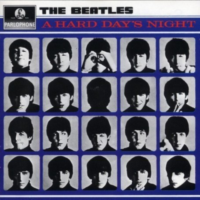
\includegraphics{hdn.png}
\caption{title}
\end{figure}

Much has been written about the chord (which, in fact, is made up of 2
guitars, one of which a 12-string, a piano and a bass) but to keep
things simple, we will accept the most prevalent thesis which states
that the notes are \(D_3, F_3, G_3, F_4, A_4, C_5\) and \(G_5\). To give
it a "wider" feeling we will add another \(D_2\) below.

In Western music, where equal temperament is used, \(A_4\) is the
reference pitch at a frequency at 440Hz. All other notes can be computed
using the formula \(f(n) = A4 \times 2^{n/12}\) where \(n\) is the
number of half-tones between \(A_4\) and the desired note. The exponent
\(n\) is positive if the note is above \(A_4\) and negative otherwise.

Each note is generated using a separate Karplus-Strong algorithm. We try
to mix the different "instruments" by assigning a different gain to each
note. Also, we sustain Paul's D note on the bass a bit longer by
changing the corresponding decay factor.

    \begin{Verbatim}[commandchars=\\\{\}]
{\color{incolor}In [{\color{incolor}19}]:} \PY{k}{def} \PY{n+nf}{freq}\PY{p}{(}\PY{n}{note}\PY{p}{)}\PY{p}{:}
             \PY{c+c1}{\PYZsh{} general purpose function to convert a note  in standard notation }
             \PY{c+c1}{\PYZsh{}  to corresponding frequency}
             \PY{k}{if} \PY{n+nb}{len}\PY{p}{(}\PY{n}{note}\PY{p}{)} \PY{o}{\PYZlt{}} \PY{l+m+mi}{2} \PY{o+ow}{or} \PY{n+nb}{len}\PY{p}{(}\PY{n}{note}\PY{p}{)} \PY{o}{\PYZgt{}} \PY{l+m+mi}{3} \PY{o+ow}{or} \PYZbs{}
                 \PY{n}{note}\PY{p}{[}\PY{l+m+mi}{0}\PY{p}{]} \PY{o}{\PYZlt{}} \PY{l+s+s1}{\PYZsq{}}\PY{l+s+s1}{A}\PY{l+s+s1}{\PYZsq{}} \PY{o+ow}{or} \PY{n}{note}\PY{p}{[}\PY{l+m+mi}{0}\PY{p}{]} \PY{o}{\PYZgt{}} \PY{l+s+s1}{\PYZsq{}}\PY{l+s+s1}{G}\PY{l+s+s1}{\PYZsq{}}\PY{p}{:}
                 \PY{k}{return} \PY{l+m+mi}{0}
             \PY{k}{if} \PY{n+nb}{len}\PY{p}{(}\PY{n}{note}\PY{p}{)} \PY{o}{==} \PY{l+m+mi}{3}\PY{p}{:}
                 \PY{k}{if} \PY{n}{note}\PY{p}{[}\PY{l+m+mi}{1}\PY{p}{]} \PY{o}{==} \PY{l+s+s1}{\PYZsq{}}\PY{l+s+s1}{b}\PY{l+s+s1}{\PYZsq{}}\PY{p}{:}
                     \PY{n}{acc} \PY{o}{=} \PY{o}{\PYZhy{}}\PY{l+m+mi}{1}
                 \PY{k}{elif} \PY{n}{note}\PY{p}{[}\PY{l+m+mi}{1}\PY{p}{]} \PY{o}{==} \PY{l+s+s1}{\PYZsq{}}\PY{l+s+s1}{\PYZsh{}}\PY{l+s+s1}{\PYZsq{}}\PY{p}{:}
                     \PY{n}{acc} \PY{o}{=} \PY{l+m+mi}{1}
                 \PY{k}{else}\PY{p}{:}
                     \PY{k}{return} \PY{l+m+mi}{0}
                 \PY{n}{octave} \PY{o}{=} \PY{n+nb}{int}\PY{p}{(}\PY{n}{note}\PY{p}{[}\PY{l+m+mi}{2}\PY{p}{]}\PY{p}{)}
             \PY{k}{else}\PY{p}{:}
                 \PY{n}{acc} \PY{o}{=} \PY{l+m+mi}{0}
                 \PY{n}{octave} \PY{o}{=} \PY{n+nb}{int}\PY{p}{(}\PY{n}{note}\PY{p}{[}\PY{l+m+mi}{1}\PY{p}{]}\PY{p}{)}
             \PY{n}{SEMITONES} \PY{o}{=} \PY{p}{\PYZob{}}\PY{l+s+s1}{\PYZsq{}}\PY{l+s+s1}{A}\PY{l+s+s1}{\PYZsq{}}\PY{p}{:} \PY{l+m+mi}{0}\PY{p}{,} \PY{l+s+s1}{\PYZsq{}}\PY{l+s+s1}{B}\PY{l+s+s1}{\PYZsq{}}\PY{p}{:} \PY{l+m+mi}{2}\PY{p}{,} \PY{l+s+s1}{\PYZsq{}}\PY{l+s+s1}{C}\PY{l+s+s1}{\PYZsq{}}\PY{p}{:} \PY{o}{\PYZhy{}}\PY{l+m+mi}{9}\PY{p}{,} \PY{l+s+s1}{\PYZsq{}}\PY{l+s+s1}{D}\PY{l+s+s1}{\PYZsq{}}\PY{p}{:} \PY{o}{\PYZhy{}}\PY{l+m+mi}{7}\PY{p}{,} \PY{l+s+s1}{\PYZsq{}}\PY{l+s+s1}{E}\PY{l+s+s1}{\PYZsq{}}\PY{p}{:} \PY{o}{\PYZhy{}}\PY{l+m+mi}{5}\PY{p}{,} \PY{l+s+s1}{\PYZsq{}}\PY{l+s+s1}{F}\PY{l+s+s1}{\PYZsq{}}\PY{p}{:} \PY{o}{\PYZhy{}}\PY{l+m+mi}{4}\PY{p}{,} \PY{l+s+s1}{\PYZsq{}}\PY{l+s+s1}{G}\PY{l+s+s1}{\PYZsq{}}\PY{p}{:} \PY{o}{\PYZhy{}}\PY{l+m+mi}{2}\PY{p}{\PYZcb{}}
             \PY{n}{n} \PY{o}{=} \PY{l+m+mi}{12} \PY{o}{*} \PY{p}{(}\PY{n}{octave} \PY{o}{\PYZhy{}} \PY{l+m+mi}{4}\PY{p}{)} \PY{o}{+} \PY{n}{SEMITONES}\PY{p}{[}\PY{n}{note}\PY{p}{[}\PY{l+m+mi}{0}\PY{p}{]}\PY{p}{]} \PY{o}{+} \PY{n}{acc}
             \PY{n}{f} \PY{o}{=} \PY{l+m+mi}{440} \PY{o}{*} \PY{p}{(}\PY{l+m+mi}{2} \PY{o}{*}\PY{o}{*} \PY{p}{(}\PY{n+nb}{float}\PY{p}{(}\PY{n}{n}\PY{p}{)} \PY{o}{/} \PY{l+m+mf}{12.0}\PY{p}{)}\PY{p}{)}
             \PY{c+c1}{\PYZsh{}print note, f}
             \PY{k}{return} \PY{n}{f}
         
         
         \PY{k}{def} \PY{n+nf}{ks\PYZus{}chord}\PY{p}{(}\PY{n}{chord}\PY{p}{,} \PY{n}{N}\PY{p}{,} \PY{n}{alpha}\PY{p}{)}\PY{p}{:}
             \PY{n}{y} \PY{o}{=} \PY{n}{np}\PY{o}{.}\PY{n}{zeros}\PY{p}{(}\PY{n}{N}\PY{p}{)}
             \PY{c+c1}{\PYZsh{} the chord is a dictionary: pitch =\PYZgt{} gain}
             \PY{k}{for} \PY{n}{note}\PY{p}{,} \PY{n}{gain} \PY{o+ow}{in} \PY{n}{chord}\PY{o}{.}\PY{n}{items}\PY{p}{(}\PY{p}{)}\PY{p}{:}
                 \PY{c+c1}{\PYZsh{} create an initial random\PYZhy{}filled KS buffer the note}
                 \PY{n}{x} \PY{o}{=} \PY{n}{np}\PY{o}{.}\PY{n}{random}\PY{o}{.}\PY{n}{randn}\PY{p}{(}\PY{n+nb}{int}\PY{p}{(}\PY{n}{np}\PY{o}{.}\PY{n}{round}\PY{p}{(}\PY{n+nb}{float}\PY{p}{(}\PY{n}{Fs}\PY{p}{)} \PY{o}{/} \PY{n}{freq}\PY{p}{(}\PY{n}{note}\PY{p}{)}\PY{p}{)}\PY{p}{)}\PY{p}{)}
                 \PY{n}{y} \PY{o}{=} \PY{n}{y} \PY{o}{+} \PY{n}{gain} \PY{o}{*} \PY{n}{KS}\PY{p}{(}\PY{n}{x}\PY{p}{,} \PY{n}{N}\PY{p}{,} \PY{n}{alpha}\PY{p}{)}
             \PY{k}{return} \PY{n}{y}  
\end{Verbatim}


    \begin{Verbatim}[commandchars=\\\{\}]
{\color{incolor}In [{\color{incolor}20}]:} \PY{c+c1}{\PYZsh{} A Hard Day\PYZsq{}s Night\PYZsq{}s chord}
         \PY{n}{hdn\PYZus{}chord} \PY{o}{=} \PY{p}{\PYZob{}}
             \PY{l+s+s1}{\PYZsq{}}\PY{l+s+s1}{D2}\PY{l+s+s1}{\PYZsq{}} \PY{p}{:} \PY{l+m+mf}{2.2}\PY{p}{,} 
             \PY{l+s+s1}{\PYZsq{}}\PY{l+s+s1}{D3}\PY{l+s+s1}{\PYZsq{}} \PY{p}{:} \PY{l+m+mf}{3.0}\PY{p}{,} 
             \PY{l+s+s1}{\PYZsq{}}\PY{l+s+s1}{F3}\PY{l+s+s1}{\PYZsq{}} \PY{p}{:} \PY{l+m+mf}{1.0}\PY{p}{,} 
             \PY{l+s+s1}{\PYZsq{}}\PY{l+s+s1}{G3}\PY{l+s+s1}{\PYZsq{}} \PY{p}{:} \PY{l+m+mf}{3.2}\PY{p}{,} 
             \PY{l+s+s1}{\PYZsq{}}\PY{l+s+s1}{F4}\PY{l+s+s1}{\PYZsq{}} \PY{p}{:} \PY{l+m+mf}{1.0}\PY{p}{,} 
             \PY{l+s+s1}{\PYZsq{}}\PY{l+s+s1}{A4}\PY{l+s+s1}{\PYZsq{}} \PY{p}{:} \PY{l+m+mf}{1.0}\PY{p}{,} 
             \PY{l+s+s1}{\PYZsq{}}\PY{l+s+s1}{C5}\PY{l+s+s1}{\PYZsq{}} \PY{p}{:} \PY{l+m+mf}{1.0}\PY{p}{,} 
             \PY{l+s+s1}{\PYZsq{}}\PY{l+s+s1}{G5}\PY{l+s+s1}{\PYZsq{}} \PY{p}{:} \PY{l+m+mf}{3.5}\PY{p}{,}
         \PY{p}{\PYZcb{}}
             
         \PY{n}{IPython}\PY{o}{.}\PY{n}{display}\PY{o}{.}\PY{n}{Audio}\PY{p}{(}\PY{n}{ks\PYZus{}chord}\PY{p}{(}\PY{n}{hdn\PYZus{}chord}\PY{p}{,} \PY{n}{Fs} \PY{o}{*} \PY{l+m+mi}{4}\PY{p}{,} \PY{l+m+mf}{0.995}\PY{p}{)}\PY{p}{,} \PY{n}{rate}\PY{o}{=}\PY{n}{Fs}\PY{p}{)}
\end{Verbatim}


\begin{Verbatim}[commandchars=\\\{\}]
{\color{outcolor}Out[{\color{outcolor}20}]:} <IPython.lib.display.Audio object>
\end{Verbatim}
            
    Close enough, no? (Check
\href{https://upload.wikimedia.org/wikipedia/en/c/c4/A_Hard_Day's_Night_opening_chord.ogg}{here}).
You can now play around with other famous chords, try for instance the
"Mystic Chord" by Scriabin, whose notes are
\(C_3, F^{\sharp}_3, B^{\flat}_3, E_4, A_4, D_5\).

    \subsection{Final Quiz}\label{final-quiz}

How would you describe what's happening here?

    \begin{Verbatim}[commandchars=\\\{\}]
{\color{incolor}In [{\color{incolor}21}]:} \PY{n}{a} \PY{o}{=} \PY{n}{np}\PY{o}{.}\PY{n}{random}\PY{o}{.}\PY{n}{rand}\PY{p}{(}\PY{l+m+mi}{100}\PY{p}{)}
         \PY{n}{b} \PY{o}{=} \PY{n}{np}\PY{o}{.}\PY{n}{random}\PY{o}{.}\PY{n}{rand}\PY{p}{(}\PY{l+m+mi}{80}\PY{p}{)}
         \PY{n}{c} \PY{o}{=} \PY{n}{np}\PY{o}{.}\PY{n}{concatenate}\PY{p}{(}\PY{p}{(}\PY{n}{a}\PY{p}{,} \PY{n}{a}\PY{p}{,} \PY{n}{a}\PY{p}{,} \PY{n}{a}\PY{p}{)}\PY{p}{)} \PY{o}{+} \PY{n}{np}\PY{o}{.}\PY{n}{concatenate}\PY{p}{(}\PY{p}{(}\PY{n}{b}\PY{p}{,} \PY{n}{b}\PY{p}{,} \PY{n}{b}\PY{p}{,} \PY{n}{b}\PY{p}{,} \PY{n}{b}\PY{p}{)}\PY{p}{)}
         
         \PY{n}{IPython}\PY{o}{.}\PY{n}{display}\PY{o}{.}\PY{n}{Audio}\PY{p}{(}\PY{n}{KS\PYZus{}1}\PY{p}{(}\PY{n}{c}\PY{p}{,} \PY{n}{Fs} \PY{o}{*} \PY{l+m+mi}{2}\PY{p}{)}\PY{p}{,} \PY{n}{rate}\PY{o}{=}\PY{n}{Fs}\PY{p}{)}
\end{Verbatim}


\begin{Verbatim}[commandchars=\\\{\}]
{\color{outcolor}Out[{\color{outcolor}21}]:} <IPython.lib.display.Audio object>
\end{Verbatim}
            

    % Add a bibliography block to the postdoc
    
    
    
    \end{document}
